\documentclass{beamer}
\setbeamercovered{transparent}
\usepackage{epstopdf}
\usepackage{listings}
\usepackage{lipsum}
\usepackage{subfig}
\usepackage{algorithm}
\usepackage{algorithmicx}
\usepackage{cite}
\usepackage{lipsum}
\usepackage{amssymb}
\usepackage{color}
\usepackage{IEEEtrantools}
\usepackage{booktabs}
\usepackage{texpower}
\usepackage{amsmath}
\usepackage{caption}
\usepackage{multirow}
\usepackage{graphicx}
\newtheorem{Key points}{Key points}
\newtheorem{Summary}{Summary}
\usepackage{dblfloatfix}
%\usepackage{adjustbox}
%\usepackage{animate}
%\usepackage{movie15}
%\usepackage{subfig}
%\newtheorem{Definition}{Definition}
%\usepackage[font={small}]{caption}
\usepackage{beamerthemeshadow}
\newcommand\Fontvi{\fontsize{5}{6.2}\selectfont}
\newcommand\Fontvia{\fontsize{6}{7.2}\selectfont}
\newcommand\Fontviaa{\fontsize{8}{7.2}\selectfont}
\usepackage{listings}
\lstset{language=C++,
                keywordstyle=\color{blue},
                stringstyle=\color{red},
                commentstyle=\color{magenta},
                morecomment=[l][\color{magenta}]{\#},
                numbers=left,
                escapeinside=||
}

%\captionsetup{font=scriptsize,labelfont=scriptsize}
 \usetheme{Antibes}%PaloAlto
\begin{document}
\title[Lecture 4]{Data Structures} 
\author[]{Ahsan Ijaz}
\date{}
 \frame{\titlepage}
% \AtBeginSection[]
% {
% \begin{frame}<beamer>{Table of Contents}
% \tableofcontents[currentsection,currentsubsection, 
%     hideothersubsections, 
%     sectionstyle=show/shaded,
% ]
% \end{frame}
% }

\section{Linked List}
 \frame{\frametitle{Linked List}
   \begin{itemize}
   \item A linked list is a data structure which can 
change during execution.
\item Successive elements are connected by pointers.Last element points to NULL.
\item It can grow or shrink in size during execution of 
a program.
\item It does not waste memory space.
   \end{itemize}
}
\frame{\frametitle{Linked List}
  \begin{figure}
    \centering
         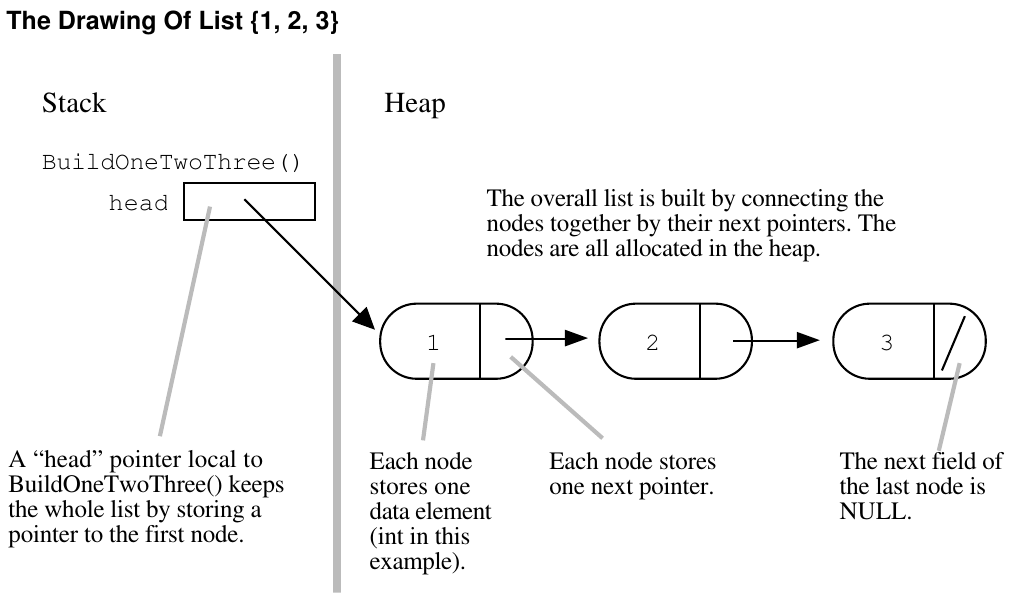
\includegraphics[width=1\columnwidth]{linkedlist}
    \caption{Linked List}
  \end{figure}
}

\begin{frame}[fragile]
  \frametitle{Basic Building Block- Self referential Class}
Self referential class containing data member and a pointer for next class of same type.
\begin{lstlisting}
class Node
{
public:
  int data;
  Node *next;
  Node(int a, Node *b)
  {
    data=a;
    next=b;
  }
};
\end{lstlisting}
\end{frame}

\begin{frame}[fragile]
  \frametitle{Linked List Implementation}
  \begin{itemize}
  \item Must know the pointer to the first element of 
the list (called start, head, etc.)
  \end{itemize}
\Fontviaa
\begin{lstlisting}
class linkedlist
{
private:
  Node *head;
public:
  void addnode(int);
  void deletenode(int);
  void insertnode(int);
  void printnode();
  linkedlist()
  {
    head=NULL;
  }
};
\end{lstlisting}
\end{frame}
\subsection{Delete Node}
\begin{frame}[fragile]
  \frametitle{Deletion}
  \begin{itemize}
  \item Get the Node prior of deletion Node (prevnode).
  \item Get the Node next of deletion Node  (nextnode).
  \item Assign address of nextnode to the next pointer of prevnode. 
  \item Delete the dynamically allocated deletion node (delnode).
  \end{itemize}
\end{frame}

\frame{\frametitle{Illustration of delete}
  \begin{figure}
    \centering
         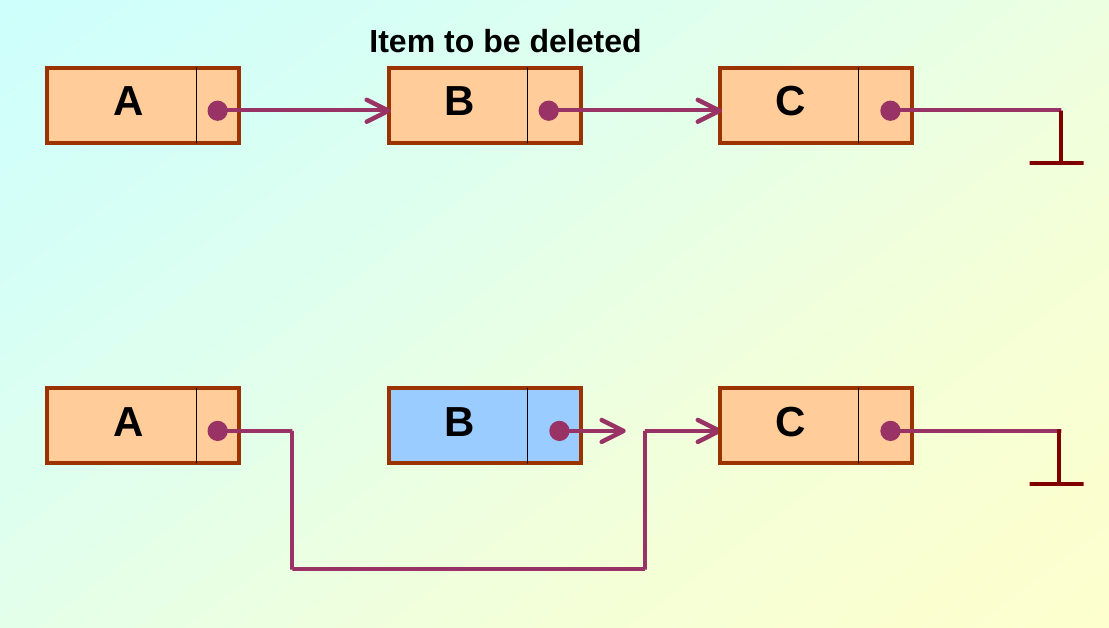
\includegraphics[width=1\columnwidth]{del.png}
    \caption{Deleting a Node}
  \end{figure}
}

\begin{frame}[fragile]
  \frametitle{Implementation of Delete}
\Fontviaa
\begin{lstlisting}
void linkedlist:: deletenode(int index)
  {
    Node *n;    //Dummy variable for traveling through llist
    Node *delnode;   //Node to be deleted
    Node *prevnode;  //Previous node
    Node *nextnode;  //Next Node
    n=head;
for (int i = 1; i < index; i++) //Index is the node which we want deleted
  {
    if(i==index-1)
      {prevnode=n;}
    n=n->next;    //Main line used to travel
  }
delnode=n;
nextnode=delnode->next;
 prevnode->next=nextnode;
 delete delnode;
  }
\end{lstlisting}
\end{frame}
\subsection{Insert Node}
\begin{frame}
  \frametitle{Insertion of Node}
  \begin{itemize}
  \item Create a new node with the required data.
  \item The next pointer of the new node is set to link 
it to the item which is to follow it in the list.
  \item The next pointer of the item which is to precede 
it must be modified to point to the new item.
  \end{itemize}
\end{frame}
\frame{\frametitle{Illustration of insertion}
  \begin{figure}
    \centering
         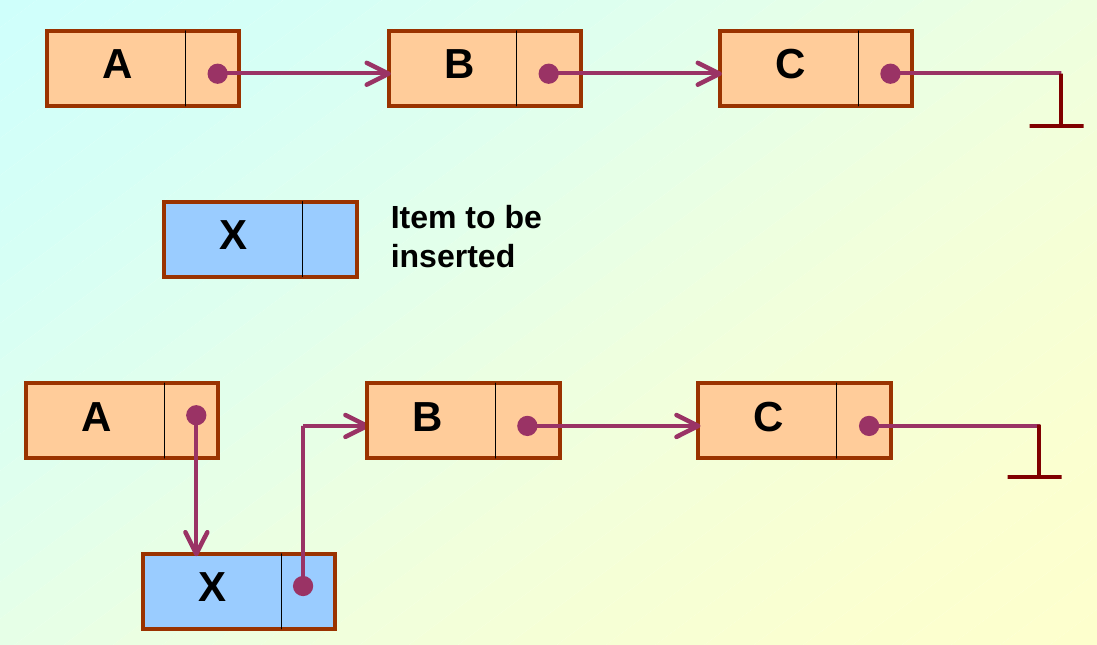
\includegraphics[width=1\columnwidth]{delete.png}
    \caption{Inserting a Node}
  \end{figure}
}
\begin{frame}
  \frametitle{Implementation of Insertion}
  \begin{center}
  \huge{LMS Assignment to be submitted by Friday}    
  \end{center}
\end{frame}
\subsection{Adding Node at end (pushback)}
\begin{frame}[fragile]
  \frametitle{Add Node Function}
\Fontviaa
\begin{lstlisting}
void linkedlist::addnode(int val)
  {
    Node *n;
    n=head;
    if(head==NULL)  //This means list contains no elements
      {
	head=new Node(val,NULL); //insert value 'val' in head
      }
    else{
    while(n->next!=NULL)//loop while next pointer of node is valid
     {
      n=n->next;  //Go through the list until last node is reached
     }
    n->next=new Node(val,NULL); //Create a new node here
    }
  }
\end{lstlisting}
\end{frame}
\subsection{}
\begin{frame}[fragile]
  \frametitle{Print Function}
\Fontviaa
\begin{lstlisting}
void linkedlist:: printnode()
  {Node *n;
    n=head;
    while(n!=NULL) //loop while n is valid 
      {
     cout<<"Data = "<<n->data<<endl; //display data in n
     n=n->next;	//travel to next point of list
      }

  }
\end{lstlisting}
\end{frame}
\subsection{Customized Linked Lists}
\begin{frame}[fragile]
The pointer from the last element in the list points
back to the first element.
  \frametitle{Circular Linked List}
  \begin{figure}
    \centering
         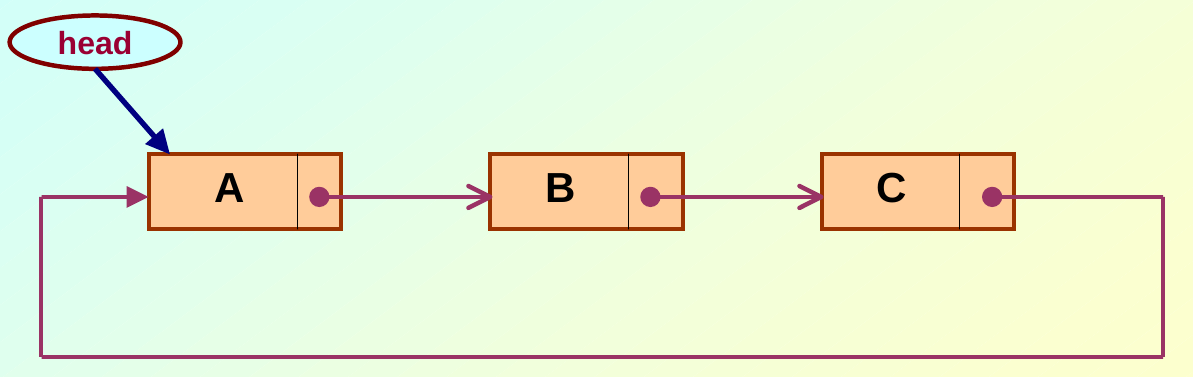
\includegraphics[width=1\columnwidth]{circle.png}
    \caption{Circular Linked List}
  \end{figure}
\begin{lstlisting}
last->next=head;
\end{lstlisting}
\end{frame}
\begin{frame}[fragile]
  \frametitle{Doubly linked List}
    \begin{figure}
    \centering
         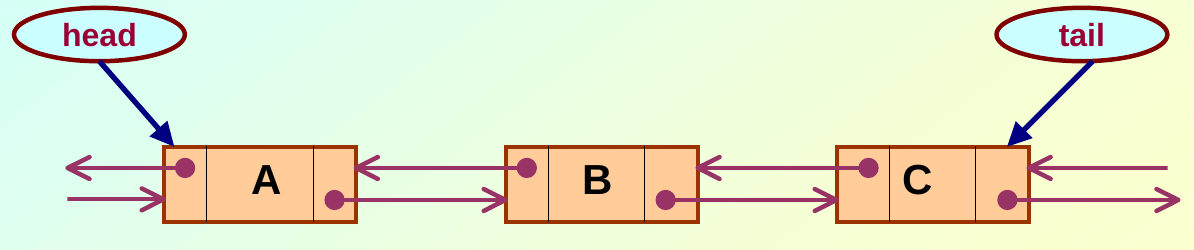
\includegraphics[width=1\columnwidth]{double.png}
    \caption{Double linked list}
  \end{figure}
\begin{lstlisting}
Node *previous; // This should be part of
                // self referential class
\end{lstlisting}
\end{frame}
\begin{frame}[fragile]
\frametitle{Queue Implementation using linked list }
\begin{center}
\huge{Ideas??}
\end{center}
\begin{lstlisting}
void pushback(int value);
Node* popfront();
\end{lstlisting}
    \begin{figure}
    \centering
         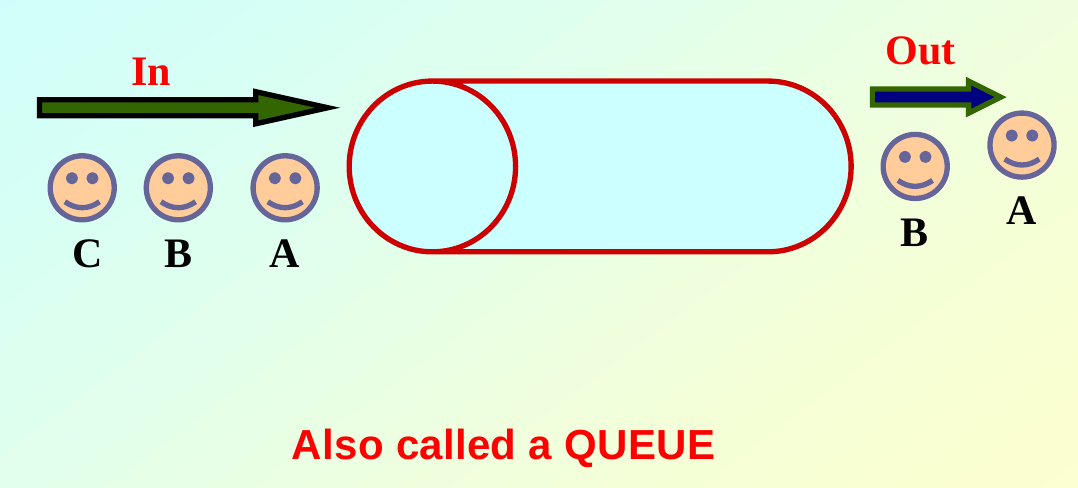
\includegraphics[width=0.5\columnwidth]{queue.png}
    \caption{Queue}
  \end{figure}
\end{frame}

\begin{frame}[fragile]
\frametitle{Stack Implementation using linked list}
\begin{lstlisting}
void pushback(int value);
Node* popback();
\end{lstlisting}
    \begin{figure}
    \centering
         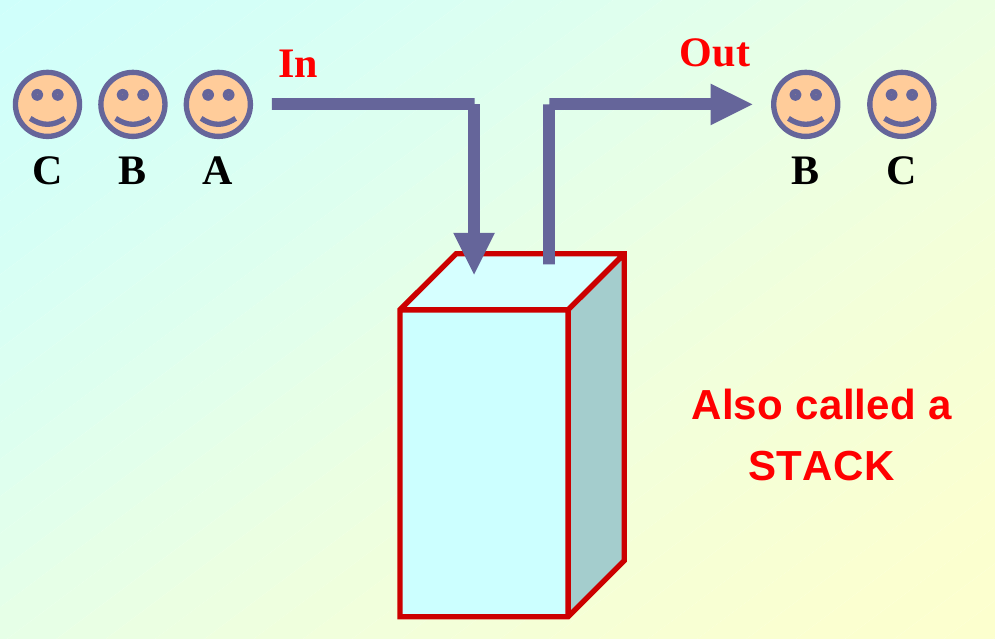
\includegraphics[width=0.51\columnwidth]{stack.png}
    \caption{Stack Implementation}
  \end{figure}
\end{frame}

\end{document}